\documentclass{article}

\usepackage{fullpage}
\usepackage{amsmath}
\usepackage{graphicx}
\usepackage[utf8]{inputenc}
\usepackage{pdfpages}

\title{Examen final de Cálculo Diferencial}
\author{M. en C. Reinaldo Arturo Zapata Peña}

\begin{document}
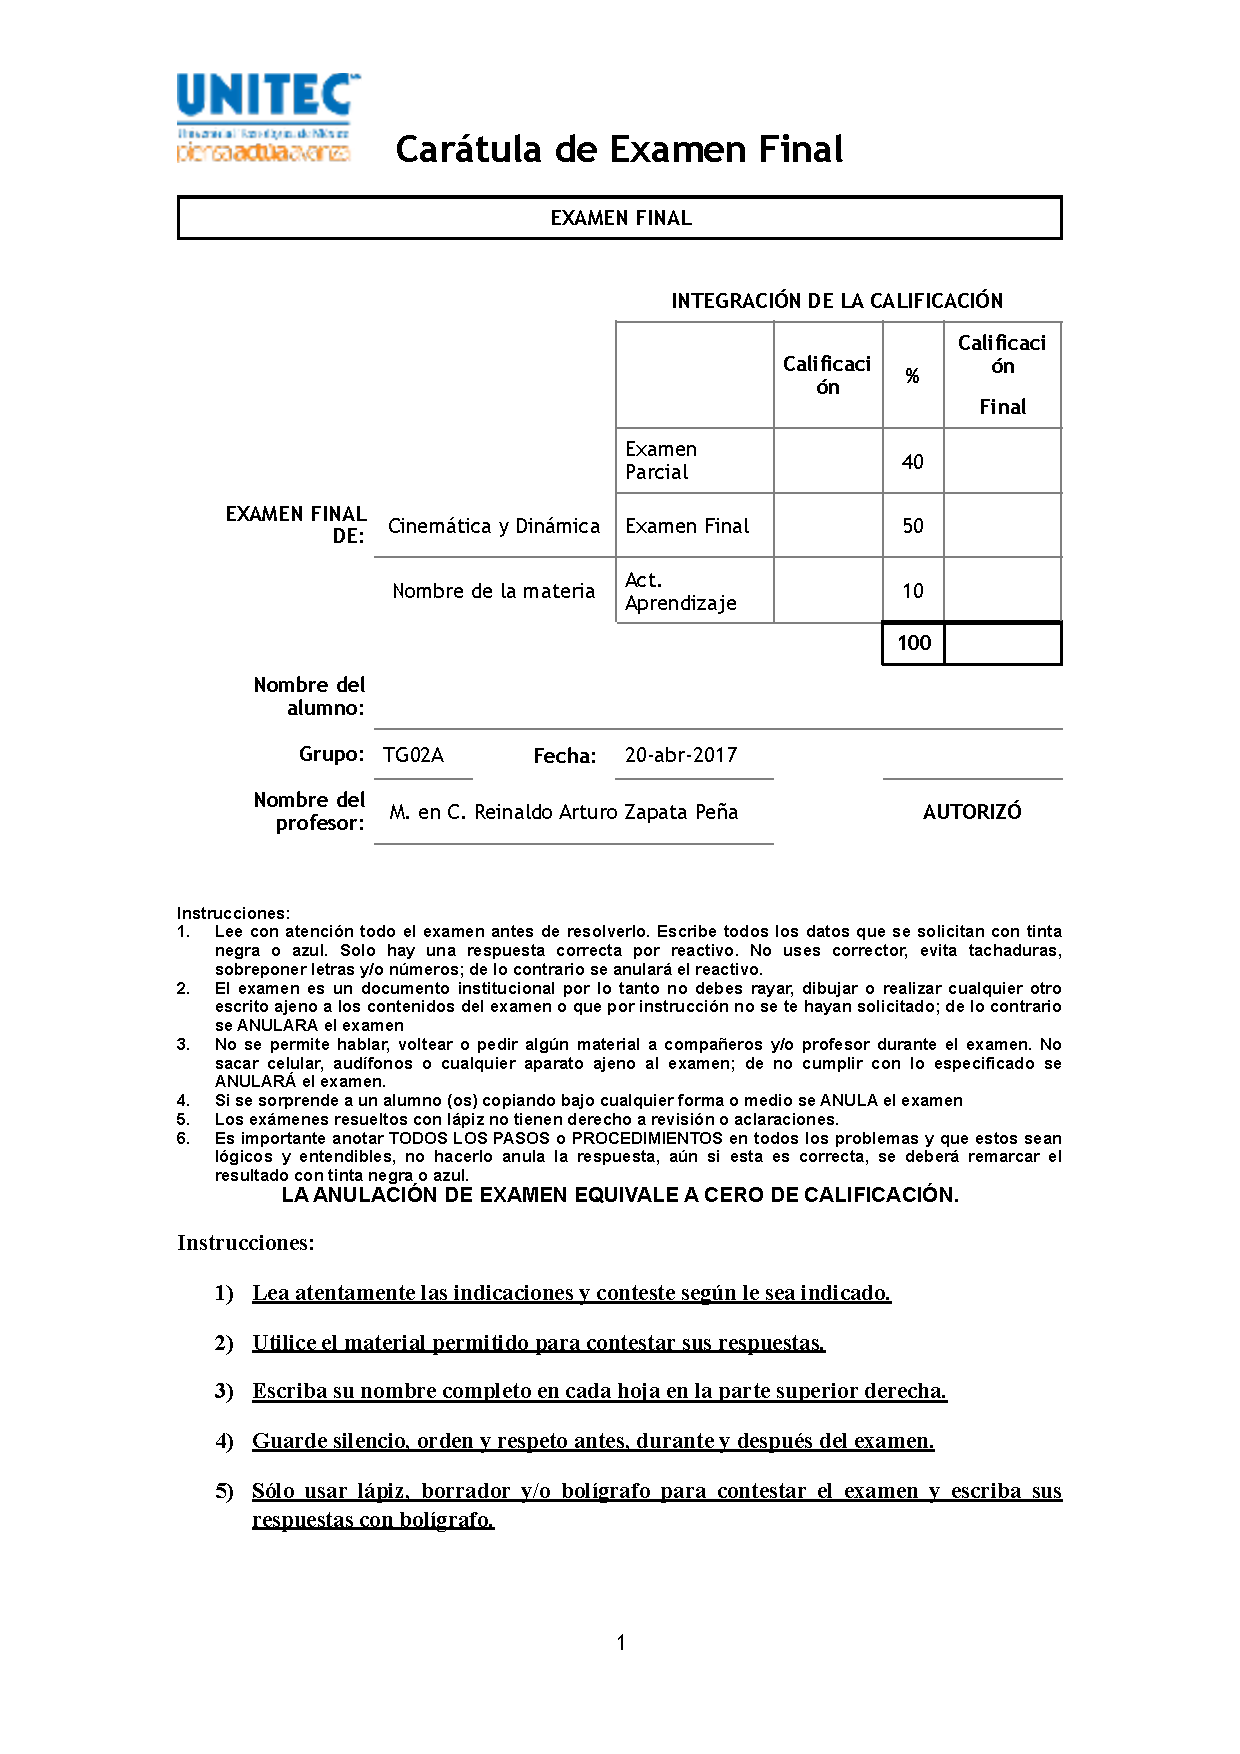
\includepdf[pages=-]{car-final-cin}

\section{Teoría} % (fold)
\label{sec:teoria}

\begin{enumerate}

\item Explique qu\'e enuncia la segunda ley de Newton y escriba la ecuaci\'on
correspondiente

\item Sean los vectores 
\begin{align}
\mathbf{A} = A_{x}\mathbf{\hat{i}} +
A_{y}\mathbf{\hat{j}} + A_{z}\mathbf{\hat{k}} \\
\mathbf{B} = B_{x}\mathbf{\hat{i}} + B_{y}\mathbf{\hat{j}} +
B_{z}\mathbf{\hat{k}}
\end{align}
¿Cuál es la diferencia entre el producto punto $\mathbf{A} \cdot \mathbf{B}$ y
el producto cruz $\mathbf{A} \times \mathbf{B}$? 

¿Qué da como resultado el producto cruz si los vectores son paralelos? 

Escriba además los elementos del producto vectorial $\mathbf{A}\times
\mathbf{B}$.

\item Considere los dos tipos de choques, elástico e inelástico. Explique que
sucede con los procesos de conservación de momento lineal y conservación de
energía cinética. 

Analizando un choque inelástico tipo \emph{Hollywood} en el que un villano
recibe un impacto de bala, ¿es posible que el sistema villano-bala salgan
volando después del impacto como lo muestran en las películas de acción?
Justifique su respuesta.

\item Partiendo de las ecuaciones de movimiento lineal, 
\begin{align}
x_{f} - x_{i} &= v_{i}t + \frac{1}{2}at^{2}, \\
v_{f} - v_{i} &= at, \\
v_{f}^{2} - v_{i}^{2} &= 2a(x_{f} - x_{i}),
\end{align}
escriba las correspondientes ecuaciones de movimiento angular.

\item Explique a que hace referencia el concepto de momento de inercia
rotacional. ¿De qué depende el momento de inercia rotacional de un objeto?

\item Dadas las ecuaciones escalar y vectorial para la torca,
\begin{align}
\tau &= rF \sin \theta = I\alpha, \\
\boldsymbol{\tau} &= \boldsymbol{r} \times \boldsymbol{F},
\end{align}
explique a qué hace referencia cada una de sus variables.

\item Explique el concepto de módulo de elasticidad. Explique los módulos de
elasticidad de Young, Shear y Bulto y relaciónelos con las siguientes tres
ecuaciones colocando las letras $Y$, $S$ y $B$ según corresponda
\begin{align}
\qquad &=  \frac{F/A}{\Delta L/L_{i}}, \\
\qquad &= -\frac{\Delta F/A }{\Delta V / V_{i}} 
= -\frac{\Delta P}{\Delta V / V_{i}}, \\
\qquad &=  \frac{F/A}{\Delta x / h}. 
\end{align}

\end{enumerate}

% section teoria (end)


\section{Problemas} % (fold)
\label{sec:problemas}

\begin{enumerate}

\item Se arroja un proyectil desde el suelo con una velocidad inicial
$v_{i}=30$\,m/s a un \'angulo de 30$^{\circ}$. Calcule el tiempo de vuelo.
Calcule la distancia $x$ que recorre el proyectil antes de golpear el suelo.
¿Cuál es la velocidad final $v_{yf}$ en la dirección $y$ justo antes del
impacto?

\item Un disco rotatorio parte del reposo y requiere 3.0\,s para completar 37.0
revoluciones. Su velocidad angular al final de este intervalo de tiempo es
98.0\,rad/s. ¿Cuál es la aceleración angular (constante) del disco?

\item Se construye un proyectil que se puede dividir a la mitad durante el
vuelo mediante un control remoto. Dicho proyectil es lanzado de forma vertical
a con una velocidad inicial $v_{yi}=19$m/s. Después de un tiempo $t=3$\,s el
control es accionado y cada mitad del proyectil adquiere una velocidad $v_{x} =
\pm5$\,m/s. Determine \emph{a}) Si el proyectil está subiendo, bajando o está
en el punto mas alto de la trayectoria, \emph{b}) El tiempo de vuelo restante
antes de golpear el suelo, \emph{c}) la distancia $\pm x$ que recorren las
mitades desde su posición original.

\item Un hombre de 78\,Kg corre con una velocidad de 7.5\,m/s hacia un trineo, 
que se encuentra sobre un lago congelado, con el fin de deslizarse sobre él. Si
el trineo tiene una masa de 7.5\,Kg, determine la velocidad a la que se mueven
el hombre y el trineo si se puede despreciar la fricción.

\item Una barra uniforme de longitud $L$ y masa $m$ está sujeto en uno de sus
extremos a una bisagra sin fricción siendo libre de rotar en el plano vertical.
La barra es liberada desde el reposo cuando forma una ángulo $\theta =
-10^{\circ}$  respecto al eje positivo $x$. ¿Cuál es la aceleración angular
inicial de la barra y la aceleración en el extremo opuesto a la bisagra?
Utilice $I= \frac{1}{3}mL^{2}$

\item Una de las vigas de soporto de un edificio, hecha de acero, soporta una
masa de $m=2,000$\,Kg. Si se tiene que su área de sección transversal es
$A=2000\,\text{cm}^{2}$, su longitud es $L=6$\,m y su módulo de Young es $20
\times 10^{10}$\,N/m$^{2}$, calcule la compresión $\Delta L$ de dicha viga.

\end{enumerate}
% section problemas (end)

%%%%%%%%%%%%%%%%%%%%%%%%%%%%%%%%%%%%%%%%%%%%%%%%%%%%%%%%%%%%%%%%%%%%%%%%%%%%%%%
%%%%%%%%%%%%%%%%%%%%%%%%%%%%%%%%%%%%%%%%%%%%%%%%%%%%%%%%%%%%%%%%%%%%%%%%%%%%%%%

\clearpage
\setcounter{section}{0}

\begin{center}
{\sc \huge Respuestas}
\end{center}

\section{Teoría} % (fold)
\label{sec:resteoria}


\begin{enumerate}
\item La aceleración de un objeto es directamente proporcional a la fuerza neta
que actúa sobre él e inversamente proporcional a su masa:
\begin{equation*}
F=ma.
\end{equation*}

\item El producto punto produce un escalar que sólo tiene magnitud mientras que
el producto cruz produce un vector perpendicular al plano formado por los
vectores en cuestión.

Si los vectores son paralelos el resultado es cero.

\begin{align*}
\mathbf{A} \times \mathbf{B} = 
(A_{y}B_{z} - A_{z}B_{y})\, \mathbf{\hat{i}} + 
(A_{z}B_{x} - A_{x}B_{z})\, \mathbf{\hat{j}} + 
(A_{x}B_{y} - A_{y}B_{x})\, \mathbf{\hat{k}}
\end{align*}

\item Para ambos casos se cumple la conservación de momento mientras que la
mientras que la conservación de energía cinética se cumple solamente para el
caso de la coalición inelástica puedes en la colisión inelástica parte de la
energía se transforma en calor.

Para el caso del disparo, el momento que lleva la bala no es suficientemente
grande como para lanzar a una persona por el aire. Esto se debe a que la masa
de la bala es muy pequeña.

\item Ecuaciones de movimiento angular:
\begin{align}
\theta_{f} - \theta_{i} &= \omega_{i}t + \frac{1}{2}\alpha t^{2}, \\
\omega_{f} - \omega_{i} &= \alpha t, \\
\omega_{f}^{2} - \omega_{i}^{2} &= 2\alpha (\theta_{f} - \theta_{i}).
\end{align}

\item El momento de inercia rotacional hace referencia a la resistencia de un
objeto a ser rotado a través de un eje. El momento de inercia rotacional de un
objeto depende de su masa Y de la distribución de dicha masa alrededor del eje
que va a ser rotado.

\item Variables de la torca:\\
$\tau$: torca\\
$r$: radio de aplicación de la fuerza\\
$F$: fuerza aplicada\\
$\theta$: ángulo formado entre $r$ y $F$\\
$I$: momento de inercia rotacional\\
$\alpha$: aceleración angular\\

\item Los módulos de elasticidad expresan que tanto de formación sufre un
objeto al momento de que se le aplica una fuerza.

\begin{align*}
Y &=  \frac{F/A}{\Delta L/L_{i}}, \\
B &= -\frac{\Delta F/A }{\Delta V / V_{i}} 
= -\frac{\Delta P}{\Delta V / V_{i}}, \\
S &=  \frac{F/A}{\Delta x / h}. 
\end{align*}

\end{enumerate}
% section resteoria (end)

\section{Problemas} % (fold)
\label{sec:problemas}

\begin{enumerate}

\item Tiro parabólico:
\begin{align*}
v_{ix} &= v_{i} \cos \theta \\
v_{iy} &= v_{i}\sin \theta \\
t &= -\frac{2v_{iy}}{g} = 3.06 \text{\,s} \\
x_{f} &= v_{ix}t = 79.50 \text{\,m}
\end{align*}

\item Disco rotatorio
\begin{align*}
\theta_{f} &= 37 \text{\,rev} = 232.5 \text{\,rad} \\
\alpha &= \frac{\omega_{f}^{2}}{2 \theta_{f}} = 
\end{align*}




\end{enumerate}
% section problemas (end)

\end{document}
